\documentclass[a4paper,14pt]{extarticle}
\usepackage{geometry}
\usepackage[T1]{fontenc}
\usepackage[utf8]{inputenc}
\usepackage[english,russian]{babel}
\usepackage{amsmath}
\usepackage{amsthm}
\usepackage{amssymb}
\usepackage{fancyhdr}
\usepackage{setspace}
\usepackage{graphicx}
\usepackage{colortbl}
\usepackage{tikz}
\usepackage{pgf}
\usepackage{subcaption}
\usepackage{listings}
\usepackage[colorlinks, linkcolor=blue, urlcolor=blue]{hyperref}
\usepackage{indentfirst}
\graphicspath{{images/}}%путь к рисункам

\makeatletter
\renewcommand{\@biblabel}[1]{#1.} % Заменяем библиографию с квадратных скобок на точку:
\makeatother

\geometry{left=2.5cm}% левое поле
\geometry{right=1.5cm}% правое поле
\geometry{top=1.5cm}% верхнее поле
\geometry{bottom=1.5cm}% нижнее поле
\renewcommand{\baselinestretch}{1.5} % междустрочный интервал

\newcommand{\bibref}[3]{\hyperlink{#1}{#2 (#3)}} % biblabel, authors, year

\renewcommand{\theenumi}{\arabic{enumi}}% Меняем везде перечисления на цифра.цифра
\renewcommand{\labelenumi}{\arabic{enumi}}% Меняем везде перечисления на цифра.цифра
\renewcommand{\theenumii}{.\arabic{enumii}}% Меняем везде перечисления на цифра.цифра
\renewcommand{\labelenumii}{\arabic{enumi}.\arabic{enumii}.}% Меняем везде перечисления на цифра.цифра
\renewcommand{\theenumiii}{.\arabic{enumiii}}% Меняем везде перечисления на цифра.цифра
\renewcommand{\labelenumiii}{\arabic{enumi}.\arabic{enumii}.\arabic{enumiii}.}% Меняем везде перечисления на цифра.цифра


\begin{document}
    \begin{titlepage}
    \newpage

    {\setstretch{1.0}
    \begin{center}
        Федеральное государственное автономное образовательное учреждение высшего образования «Национальный исследовательский университет «Высшая школа экономики»
        \\
        \bigskip
        Факультет компьютерных наук \\
        Основная образовательная программа \\
        Прикладная математика и информатика \\
    \end{center}
    }

    \vspace{8em}

    \begin{center}
    {\Large ГРУППОВАЯ КУРСОВАЯ РАБОТА}
        \\
        \textsc{\textbf{
        Программный проект на тему
        \linebreak
        "Решения на основе компьютерного зрения для проектов в городской среде"}}
    \end{center}

    \vspace{2em}

    {\setstretch{1.0}
    \hfill\parbox{16cm}{
    \hspace*{5cm}\hspace*{-5cm}Выполнили студент группы 171, 3 курса,\\
    Биршерт Алексей Дмитриевич,\\
    Шабалин Александр Михайлович\\

    \hspace*{5cm}\hspace*{-5cm}Руководитель КР:\\
    старший преподаватель Соколов Евгений Андреевич
    \\

    %\hspace*{5cm}\hspace*{-5cm}Куратор:\hfill < степень>, <звание>, <ФИО полностью>\\

    \hspace*{5cm}\hspace*{-5cm}Консультант:\\
    научный сотрудник Лобачева Екатерина Максимовна\\
    }
    }

    \vspace{\fill}

    \begin{center}
        Москва 2020
    \end{center}

\end{titlepage}
    \newpage

    {
        \hypersetup{linkcolor=black}
        \tableofcontents
    }

    \newpage

    \begin{abstract}
        Автоматическое предсказание пола и возраста человека по фотографиям, полученным в самых разных условиях -
        это важная и сложная задача, находящая применение во многих областях жизнедеятельности людей.
        В своем проекте мы стремились воплотить подход к решению этой задачи, основанный на сверточных нейронных сетях.
        Свое решение мы разбили на две составных части - детектирование лица человека и ключевых точек на его лице
        и дальнейшее предсказание пола и возраста по признакам лица.
        \par Для детектирования мы используем архитектуру RetinaFace с предобученным на ImageNet-1000 ResNet-18 в качестве основой модели.
        В качестве обучающих данных мы используем датасет WIDER FACE с добавленными к нему пятью ключевыми точками для каждого лица.
        На тестовой выборке наш детектор получает значение метрики Precision равное 83\%.
        \par Для классификации найденных лиц мы используем модель на основе двух предобученных на ImageNet-1000 ResNet-18.
        В качестве обучающих данных мы испольуем датасеты IMDB-WIKI-101 и FGNET\@.
        В качестве тестовых данных мы используем датасет Adience, наша модель получает для возраста значение метрики
        Exact-accuracy 45\% и значение метрики One-off-accuracy 80\%, для пола значение метрики Accuracy 85\%.
        \par В итоге мы получили рабочую модель, способную обрабатывать большие массивы фотографий,
        детектировать на них людей и предсказывать для их пол и возраст в автоматическом режиме.
        Ссылка на гитхаб с проектом - \url{https://github.com/birshert/age_gender_classification}.
        \\
        \\
        \small \textbf{\textit{Ключевые слова---}}Определение возраста и пола, Детектирование лиц, Компьютерное зрение, Глубокое обучение \\
        Automatically predicting real age and gender from face images acquired in unconstrained conditions
        is an important and challenging task in many real-world applications.
        In our project we intended to construct an approach to predicting a person's real age and gender from photograph
        based on convolutional neural networks.
        Our solution is divided into solving two separate subtasks - detecting one's face and it's landmarks and
        further age and gender estimation based on facial features.
        \par For face detection we use RetinaFace architecture with a pretrained on ImageNet-1000 ResNet-18 as a backbone.
        For training we use WIDER FACE dataset with added five facial landmarks for every face.
        On testing subset we achieve 83\% Precision result.
        \par For real age and gender estimation we use a model based on two pretrained on ImageNet-1000 ResNet-18.
        For training we use IMDB-WIKI-101 dataset and FGNET dataset.
        For testing we use Adience dataset, our model achieves Exact-accuracy 45\%, One-off-accuracy 80\% for age estimation
        and 85\% Accuracy for gender prediction.
        \par As a result, we got a working model capable of processing large volumes of photos, detecting people faces on them and predicting their real age and gender in automatic mode.
        Github project link - \url{https://github.com/birshert/age_gender_classification}.
        \\
        \small \textbf{\textit{Keywords---}}Age and gender estimation, Facial detection, Computer vision, Deep learning
        \\
        \newpage
    \end{abstract}


    \section{Введение}\label{sec:введение}
    Во многих сферах деятельности требуется получать информацию о статистике про людей, проживающих на некоторой территории или пользующихся каким-либо продуктом.
    Хорошим источником такой информации являются фотографии людей, запечатлённых в определенных местах.
    Однако ручная обработка десятков тысяч фотографий в попытке получить нужные данные крайне сложна и время- и трудозатратна,
    поэтому большинство современных решений являют собой автоматическую обработку массивов фотографий,
    классифицируя людей на фотографиях по полу и возрасту с помощью методов компьютерного зрения.
    \par За время исследования проблемы классификации людей по фотографиям стало ясно, что использование алгоритмов,
    опирающихся на фиксированные выделенные людьми признаки, не приносит удовлетворительных результатов.
    Так происходит потому, что люди на фотографиях, запечатленные в неформальных условиях,
    имеют множество разных поз, форм и вариаций поворотов относительно камеры, которые не поддаются ручному анализу.
    \par Все известные подходы к классификации возрастных групп людей по фотографии заключаются в анализе изображения лица.
    Самые ранние~\cite{age1994} основывались на различиях в пропорциях и размерах черт лица в зависимости от возраста -
    так называемые антропометрические модели~\cite{unfiltered}.
    Все они вычисляли координаты точек на лице и в дальнейшем их анализировали.
    Более поздние и более современные методы~\cite{hassner,INDIA} опирались на использование сверточных нейронных сетей небольшой глубины.
    Самые современные подходы используют глубокие сверточные нейронные сети~\cite{DEEP}.
    \par Первые подходы к классификации пола использовали фотографии лица низкого разрешения - до 20 на 20 пикселей,
    и обучали на них различные типы классификаторов~\cite{smoll}.
    Позднее стали использовать LBP для выявления новых признаков~\cite{lbp_age},
    использовать сверточные нейронные сети~\cite{hassner,INDIA}.
    \par В ходе выполнения работы мы не будем предлагать каких-либо новых методов,
    однако мы воспользуемся рядом различных уже существующих технологий машинного обучения,
    проверив их качество при применении к нашей задаче.
    В итоге мы получим алгоритм, способный перебирать большие объемы фотографий,
    находить на них лица людей, а затем классифицировать их по полу и возрасту.
    \par Дальнейшая работа описана в следующих главах -
    Обзор литературы, Детектирование лиц, Классификация гендерных и возрастных групп, Выводы и Планы дальнейшей работы.
    "Детектирование лиц"\,выполнено Александром Шабалиным, "Классификация гендерных и возрастных групп"\,Алексеем Биршертом.
    \newpage


    \section{Обзор литературы}\label{sec:обзор-литературы}
    \subsection{Детектирование лиц}\label{subsec:детектирование-лиц}
Детектирование лиц на фотографии - одна из древнейших задач компьютерного зрения, возникшая в 1990-х годах.
Первые хорошие результаты появились в 2004 году.
Описанный в статье~\cite{face_detection} метод находил лица с помощью признаков Хаара, используя каскад детекторов, обученных алгоритмом AdaBoost.
В 2014 году в статье~\cite{face_detection2} был предложен метод, использующий Deformable Parts AgeGender (DPM).
Его идея заключается в нахождении зависимостей между подвижными частями.
Например, лицо представляется, как нечто, состоящее из глаз, носа, рта, расположенных в некотором антропоморфическом виде.
Однако все описанные методы показывали довольно плохие результаты в сложных случаях, так как опирались на ограниченный, придуманный людьми набор признаков.
Поэтому методы, основанные на сверточных нейронных сетях быстро вытеснили остальные.
Лучшие известные на данный момент подходы описаны в статье~\cite{face_detection3}.
Все из них используют нейронные сети (обычно ResNet~\cite{resnet}) для получения признаков.
Так как модель сама находит признаки и зависимости, результат получается лучше.
\par Немаловажной задачей является и выравнивание лиц.
Самый быстрый метод получить выровненное лицо - определить ключевые точки на лице и преобразовать изображение так, чтобы эти точки были на заранее определенных местах.
В статье~\cite{align} описан метод вычисления координат основных точек на лице человека - окаймляющих лицо, глаза, нос, рот и брови.
Вычисление точек происходит с помощью каскада регрессоров, обучаемых с помощью градиентного бустинга.
\par В нашей работе мы пользуемся архитектурой RetinaFace~\cite{retinaface}.
На данный момент она является state-of-the-art в задаче детектирования лиц и показывает впечатляющие результаты.
Одна из ее отличительных черт - умение предсказывать пять ключевых точек, необходимых для выравнивания изображения.

\subsection{Классификация возраста и пола}\label{subsec:классификация-возраста-и-пола}
\par Задачи определения пола и возраста человека находят применение в разных сферах жизни человека, в наружном наблюдении, в антропологии, в биометрической идентификации.
Современные подходы к этой задаче опираются на сверточные нейронные сети.
Так, например, в статье~\cite{hassner} описано решение с помощью сверточной сети небольшой глубины.
Для классификации возраста и пола используется одна и та же архитектура.
Нейронная сеть состоит из трёх свёрточных слоёв и двух полносвязных,
небольшой размер сети объясняется желанием быть физичным в распознавании лиц и нежеланием переобучиться.
Точность по классификации пола была 86.8 $\pm$ 1.4\%,
возрастных групп - 50.7 $\pm$ 5.1\% для точного попадания в группу и 84.7 $\pm$ 2.2\% для попадания в правильную или соседнюю для датасета Adience.
\par В статье~\cite{INDIA} описан алгоритм анализа лица с помощью пяти сверточных нейросетей, получающих изображения лица целиком, левого и правого глаза, носа и рта соответственно.
Итоговое решение принимается на основе выходов всех пяти нейросетей.
Нейросеть, получающая на вход всё изображение лица, имеет три сверточных слоя, прочие по два.
Точность по классификации пола достигла 89.6 $\pm$ 1.3\%,
возрастных групп - 54.3 $\pm$ 3.5\% для точного попадания в группу и 87.6 $\pm$ 1.9\% для попадания в правильную или соседнюю на датасете Adience,
что является значительным улучшением результата предыдущей статьи.
\par В статье~\ref{imdb} описан метод использования ансамбля глубоких сверточных нейронных сетей для предсказания реального возраста.
Для этого авторы статьи собрали свой собственный датасет IMDB-WIKI-101,
дообучали на нём модели с архитектурой VGG-16 предобученные на ImageNet-1000,
потом классифицировали признаки, полученные сверточной нейронной сетью с помощью двух полносвязных слоев
и использовали выход второго слоя для предсказания возраста от 0 до 100 включительно.
В процессе они использовали различные улучшения в выравнивании лиц (вращали изображение вдоль центра
и выбирали детектированное лицо с максимальным показателем уверенности модели детектирования лиц),
затем тренировали ансамбль из 20 моделей на датасете LAP~\ref{LAP} для получения оптимального результата.
В итоге им удалось получить результат MAE по возрасту 3.2 на датасете IMDB-WIKI-101.
\newpage


    \section{Детектирование лиц}\label{sec:детектирование-лиц}
    \subsection{Описание выбранного метода}\label{subsec:описание-выбранного-метода}
Для детектирования лиц была использована архитектура нейронной сети RetinaFace\cite{retinaface}.
Она состоит из двух частей: основной модели и пирамиды признаков.
Основная модель - это сверточная нейронная сеть, предназначенная для выявления признаков из изображения.
В качестве основной модели может выступать MobileNet~\cite{mobile}, VGG, ResNet и другие.
\par Идея пирамиды признаков довольно проста.
При детектировании лиц мы хотим находить лица разных размеров.
Для этого строятся две пирамиды из пяти карт признаков в каждой.
Первая получается проходом снизу в верх, а вторая - сверху вниз.
Слоями первой пирамиды являются выходы четырех слоев основной модели такие,
что размер каждого следующего выхода в два раза меньше размера предыдущего.
Так мы получаем карты разного размера, что позволяет детектировать как маленькие, так и большие лица.
Вторая пирамида необходима из-за того, что на ранних слоях сверточной сети содержится значительно меньше семантической информации,
а значит, предсказания лиц на ранних слоях менее точны и мы должны как-то компенсировать это.
Слои второй пирамиды мы получаем, проходя сверху вниз следующим образом.
Первый (верхний) слой получается с помощью наложения свертки с ядром размера 1х1 на верхний слой первой пирамиды.
Каждый следующий из пяти слоев получается путем поэлементого суммирования предыдущего слоя,
увеличенного в два раза, со сверткой размера 1х1 соответствующего слоя первой пирамиды.
Таким образом нам удается передать большим по размеру картам признаков семантическую информацию меньших карт, компенсировав ее нехватку.
Подобная передача информации от первой пирамиды также моделирует обходные связи, используемые в ResNet и улучшающие обучение модели.

Важным объектом данной архитектуры являются якори.
При детектировании лиц на карте признаков карта разбивается на сетку из регионов, каждый регион содержит в себе k прямоугольников различных форм и размеров (якорей).
Каждый якорь несет в себе предсказание об ограничивающем контуре, ключевых точках и бинарной классификации лицо/не лицо в заданном им прямоугольнике, то есть якорь содержит 4 + 10 + 2 = 16 параметров.
Предсказания получаются с помощью применения нескольких сверточных слоев с размерами ядер 5х5 и 7х7 к картам признаков второй пирамиды и конкатенированием результатов этих сверток.
Число выходных каналов этих сверток должно равняться 16, так как именно столько парамертов обозначают предсказание лица.
\\
\par В нашей реализации в качестве основной модели используется ResNet18 предобученный на ImageNet-1000~\cite{imagenet}.
Выходы четырех блоков ResNet являются четыремя картами признаков первой пирамиды,
пятая карта признаков получается наложением свертки с ядром размера 3х3 и шагом 2 на последнюю карту признаков.
Так как датасет ImageNet содержит в себе картинки с различными изображениями,
а в нашей задаче необходимо находить лица людей, мы замораживем только первый слой ResNet, а остальные дообучаем.
Выбор ResNet с 18 слоями обосновывается тем, что в нашей задаче также важна скорость работы.
С увеличением размера сверточной сети время ее работы заметно увеличивается, а качество растет не так сильно.
% TODO Это будет видно на графиках
% TODO написать о pyramid feature

\subsection{Подготовка данных и обучение}\label{subsec:подготовка-данных-и-обучение}
Для обучения модели был использован датасет WIDER FACE~\cite{wider}.
Он содержит 32,203 фотографии с 393,703 лицами на них.
Для каждого лица хранятся координаты пяти ключевый точек: две для глаз, одна для носа и две для рта,
а также координаты прямоугольной рамки, ограничивающей лицо.
В качестве аугментации мы пробовали делать случайный переворот изображения,
однако он не улучшил результаты, поэтому мы решили от него отказаться.
Входные изображения масштабируются до квадратных следующим образом: большая сторона становится равной 256,
а к меньшей добавляется нулевой отступ с двух сторон так, чтобы размер итогового изображения составлял 256 на 256.
При обучении был использован Adam оптимизатор со скоростью обучения $10^{-3}$.
Модель обучается в течение 20-ти эпох с размером батча 32.
\par Ошибка модели считается по формуле: \[L = L_{cls}(p, p^*) + 0.25 L_{box}(t, t^*) + 0.1 L_{pts}(l, l^*),\]
где $p$ - вероятность лица, $p^*$ - истинный ответ (0 или 1),
для подсчета ошибки классификатора $L_{cls}(p, p^*)$ используется софтмакс ошибка для бинарных классов классов (лицо/не лицо).\\
$t = \{t_1, t_2, t_3, t_4\}$ и $t^* = \{t^*_1, t^*_2, t^*_3, t^*_4\}$ предсказанные и истинные координаты ограничивающей рамки соответственно.
Для подсчета ошибки $L_{box}(t, t^*)$ используется функция $\text{Smooth-L}_1$ loss.
\\$l = \{l_{x1}, l_{y1}, \dots, l_{x5}, l_{y5}\}$ и $l = \{l^*_{x1}, l^*_{y1}, \dots, l^*_{x5}, l^*_{y5}\}$ предсказанные и истинные координаты ключевых точек лица.
Для подсчета ошибки $L_{pts}(l, l^*)$ так же используется $\text{Smooth-L}_1$ loss.

\subsection{Выравнивание}\label{subsec:выравнивание}
Перед передачей найденных лиц классификатору возраста и пола необходимо их выровнить.
Выравнивание производится на основе двух ключевых точек для глаз, найденных вместе с лицами.
Для этого находится угол отклонения прямой, проведенной с помощью точек глаз, от горизонтали.
После этого мы домножаем матрицу изображения на матрицу поворота таким образом, что линия глаз становится горизонтальной.
Мы не используем остальные точки, так как они избыточны, а в некоторых случаях даже мешают.
Например, расположение точек рта у улыбающегося человека и у серьезного отличаются, но это отличие не должно никак влиять на выравнивание.
Глаза же всегда располагаются на одном месте относительно лица, что позволяет их считать хорошей опорой для выравнивания.

\subsection{Эксперименты}\label{subsec:эксперименты2}
Для определения с выбором основной модели были проведены сравнения между ResNet18, ResNet50, VGG и MobileNet.
По результатам этого эксперимента выяснилось, что ResNet50 получает лучший результат,
но для предсказания ответа ему требуется гораздо больше времени, чем ResNet18.
MobileNet работает быстрее остальных, но ошибка такой модели оказывается больше остальных.
VGG показывает хороший результат, но работает медленнее всех.
В результате выбор остановился на ResNet18, потому что баланс скорости и качества детектирования лиц этой модели мы считаем оптимальным.

% TODO график сравнения с ResNet другого размера, VGG и MobileNet, сказать, что другие реснеты гораздо медленее, что для нас критично.
Для ускорения времени работы алгоритма мы пробовали уменьшать число карт признаков в пирамиде признаков,
однако в таком случае некоторые слишком большие или слишком маленькие лица переставали обнаруживаться,
что крайне негативно отражалось на результатах модели.
% TODO посмотреть, что будет при изменении числа слоев в feature pyramid, попробовать менять параметры якорей.
% TODO попробовать другой оптимизатор.
% TODO оценить качество предсказания landmarks и показать, что другие методы работают хуже.

\subsection{Результаты}\label{subsec:результаты2}
Полученная модель хорошо справляется с поставленной задачей, получая значение метрики Precision равное 83\%.
Для нашей задачи эта метрика имеет крайне важное значение, так как ты не должны классифицировать несуществующих людей.
Несмотря на то, что реализация авторов RetinaFace получала 91\%, мы считаем это хорошим результатом,
так как из-за нехватики вычислительных мощностей пришлось почти в 3 раза снизить размер стороны входного изображения,
использовать ResNet18 вместо ResNet152, а также уменьшить количество эпох обучения, что заметно сказывается на результатах работы.

\newpage

\subsection{Примеры работы модели}\label{subsec:примеры-работы-модели}
\begin{figure}[h!]
    \centering
    \begin{subfigure}[b]{1.02\linewidth}
        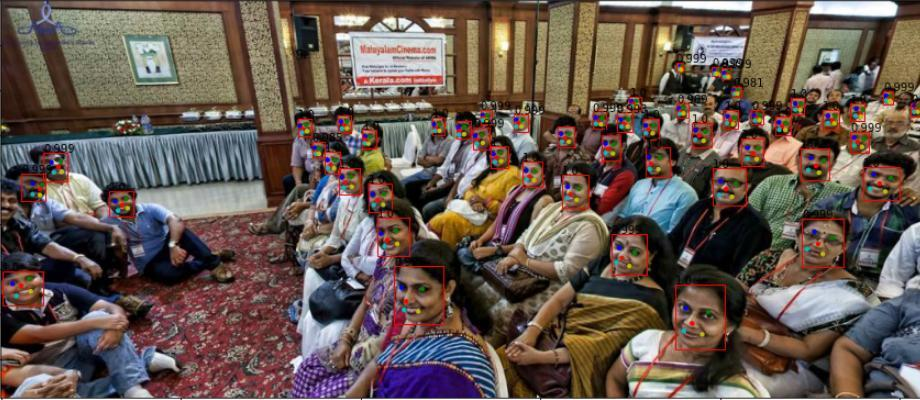
\includegraphics[width=\linewidth]{images/good1.jpg}
        \caption{Модель смогла найти 50 лиц из 61 указанного в ответе.}
    \end{subfigure}

    \centering
    \begin{subfigure}[b]{1.02\linewidth}
        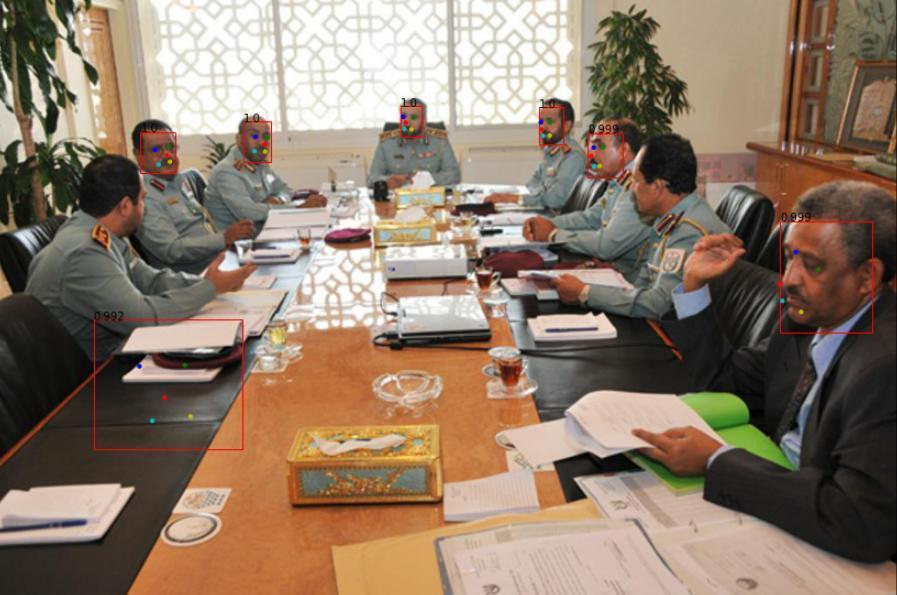
\includegraphics[width=\linewidth]{images/norm1.jpg}
        \caption{Модель хорошо справилась со своей задачей, найдя все повернутые к камере лица, однако она также выделила пустую часть стола.}
    \end{subfigure}
\end{figure}

    \newpage


    \section{Классификация гендерных и возрастных групп}\label{sec:классификация-гендерных-и-возрастных-групп}
    Эта часть выполнена Алексеем Биршертом. \\

\subsection{Описание выбранного метода}\label{subsec:описание-метода}
Для предсказания пола и возраста используются две нейронные сети, состоящие из основной и выходной моделей каждая.
В качестве основной модели используется глубокая нейронная сеть ResNet-18, без последнего полносвязного слоя.
В качестве выходной модели используется персептрон из двух полносвязных слоёв с нелинейностью ReLU и дропаутом между ними.
На вход основной модели подаются изображения 227 на 227 пикселей, 3 канала цвета - R, G, B,
выход основной модели подаётся на вход выходной модели.
Выходом нейросети будет выход выходной модели.
Первая нейронная сеть предназначена для классификации пола и имеет в выходной модели 512 и 256 входных и выходных нейронов в первом слое, 256 и 2 во втором соответственно.
Вторая нейронная сеть предназначена для классификации возраста и имеет в выходной модели 512 и 512 входных и выходных нейронов в первом слое, 512 и 101 во втором соответственно.
На вход подаются фотографии лиц людей, выделенные и выровненные с помощью модели детектирования лиц.
Предсказанный пол определяется как номер выходного нейрона соответствующей нейронной сети с максимальным значением -
первый это "женский"\,, второй "мужской".
Предсказанный возраст определяется следующим образом: сначала для вектора значений выходных нейронов
соответсвующей нейронной сети применяется преобразование софтмакс, затем значения умножаются на соответствующий
им возраст.
После вектор суммируется - получаем матожидание возраста при вероятностном распределении, выданном моделью.
\[AGE = \sum\limits_{i = 0}^{100}i \cdot softmax(x)_i, \quad softmax(x)_i = \frac{\exp(x_i)}{\sum\limits_{j =
0}^{100}\exp(x_j)}.\]

\subsection{Описание и подготовка данных}\label{subsec:описание-данных}
В качестве датасета для обучения двух вышеописанных моделей были избраны датасеты IMDB-WIKI-101~\cite{imdb_db} и FGNET~\cite{fgnet}.
Оба датасета имеют в мета-данных метки пола "женщина" или "мужчина"\, и имеют метки возраста в виде целых чисел от 0 до 100 включительно.
Распределение возраста в датасете IMDB-WIKI-101 имеет вид нормальной кривой со средним около 35 лет,
имея малое количество объектов с возрастом меньше 10 лет или больше 90.
Для увеличения количества данных с возрастом до 10 лет был избран датасет FGNET, в котором большая часть объектов это дети до 15 лет.
Для улучшения сходимости нейронных сетей была произведена предобработка всех объектов -
в итоговую выборку не были включены следующие объекты:
объекты с плохо различимыми лицами (показатель уверенности модели распознавания лиц в том, что это лицо, ниже фиксированного значения),
объекты с некорректно заполненными данными по полу/возрасту,
объекты со слишком маленькими фотографиями.
На каждом изображении было выделено и выровнено лицо.
Отступ от границы лица был поставлен на 40\%, чтобы лицо целиком оказывалось на выделенной зоне.
Итого было получено около 200 тысяч объектов, которые были в дальнейшем поделены
с сохранением баланса классов 1 к 19 на валидационную и обучающую выборки соответственно.
\par В качестве датасета для тестирования был избран датасет Adience~\cite{adience}, по которому известно большое количество результатов различных моделей.
Из него были исключены объекты с некорректным описанием пола или возраста.
Итого было получено почти 11 тысяч объектов для тестовой выборки.
В Adience метки возраста в формате 8 групп - 0: [0, 2], 1: [4, 6], 2: [8, 12], 3: [15, 20], 4: [25, 32], 5: [38, 43], 6: [48, 53], 7: [60, 100].
В связи с этим, необходимо было решить как относить к этим группам метки реального возраста от 0 до 100.
Было принято решение относить к той группе, граница которой ближе по модулю, в случае равенства относить к первой в порядке следования.

\subsection{Постановка задач обучения}\label{subsec:постановка-задач-обучения}
Задача классификации пола является задачей бинарной классификации, целевая переменная для одного объекта это число 0 или 1.
Для обучения была выбрана перекрестная энтропия - функция ошибки со следующей формулой:
\[loss(x, y) = -x_y + \log\left(\sum\limits_{j=1}^{K}\exp(x_j)\right),\] где $x$ - вектор значений выходных нейронов нейронной сети,
$y$ - целевая переменная.
Для оценки качества классификации использовались метрика доля правильных ответов, так как выборки сбалансированны по полу.
\par Задача классификации возраста является задачей многоклассовой классификации.
Если смотреть на задачу предсказания возраста по фотографии с точки зрения человека,
человек гораздо точнее способен угадать диапазон возраста, нежели точный возраст.
Поэтому задача классификации возраста была интерпретирована как задача с множественными правильными ответами -
каждому объекту может соответствовать набор правильных классов.
Целевой переменной для одного объекта служил вектор из нулей и единиц, единицы на позициях правильных классов.
Правильные классы определялись как значения возраста, которые отличаются по модулю от правильного не больше,
чем на фиксированное число, которое было гиперпараметром (далее об этом в разделе эксперименты~\ref{subsec:эксперименты}).
Для обучения была выбрана бинарная перекрестная энтропия -
\[loss(x, y) = sum(L), \quad L = \{l_1, \dots l_N\}, \quad l_i = \left(y_i \log(x_i) + (1 - y_i) \log(1 - x_i)\right),\]
где $x$ это вектор значений выходных нейронов нейронной сети после применения сигмоидного преобразования,
$y$ - целевая переменная.
Для оценки качества классификации использовались средний модуль отклонения (далее MAE)
и доля объектов, у которых MAE не превышает фиксированного числа (далее CS-5).

\subsection{Эксперименты}\label{subsec:эксперименты}
В качестве основных было рассмотрено два варианта - нейронная сеть на основе статьи~\cite{ror} и нейронная сеть на основе статьи~\cite{lstm}.
Однако стоит заметить, что анализ и использование модели из второй статьи на порядок сложнее, так как помимо сверточных нейронных сетей там используется блок LSTM,
для работы с которым необходимо иметь соответствующий опыт.
Поэтому было принято решение базировать работу на основе первой статьи, слегка упростив архитектуру.
\par Необходимо было решить вопрос выбора архитектуры базовой модели.
Всего было опробовано три различных архитектуры - MobileNet, ShuffleNet~\cite{shuffle}, ResNet.
Лучше всего себя проявила архитектура ResNet-18.
MobileNet и ShuffleNet незначительно быстрее, не смотря на реализацию, однако достаточно сильно проигрывали в качестве.
В итоге была выбрана архитектура ResNet.
\par Так как ResNet-18 предобучен на датасете ImageNet-1000, он имеет очень хорошую способность выделять признаки из изображения.
Известно, что первые (входные) сверточные слои обученных моделей очень похожи между собой даже для различных задач.
Таким образом, было решено веса первого сверточного слоя ResNet-18 взять из предобученной на ImageNet-1000 модели и заморозить в процессе обучения,
дообучая веса всех остальных слоев.
\par Вторым необходимо было решить вопрос выбора количества моделей - одна нейронная сеть из общей базовой модели и двух паралелльных выходных моделей
или две отдельные нейронные сети из основной и выходной модели.
Однако стоит заметить, что для обеих задач нейронная сеть и должна выделять признаки лица, признаки,
отвечающие за пол, несколько отличаются от признаков, которые соответствуют возрасту.
Также в силу использования функций ошибки,
которые имеют разный масштаб и решают частично разные задачи на моменте основной модели,
и сложности в подборе гиперпараметров для комбинирования этих функций ошибки,
нейронная сеть из одной общей основной модели очень плохо сходилась и достигала намного меньшего качества во всех проведенных экспериментах.
В итоге было принято решение использовать две паралелльные нейронные сети, по одной на решаемую задачу.
\par В процессе подбора гиперпараметров для обучения были выбраны следующие значения: темп обучения был выставлен на $1e-3$ для первых 40 эпох,
далее $1e-4$ для модели предсказания возраста, $1e-4$ для первых 30 эпох и $2e-5$ далее для модели предсказания пола;
коэффициент $L2$ регуляризации был установлен на $1e-3$ для обеих моделей;
размер батча был установлен в силу ограничений на память ГПУ и в качестве дополнительной регуляризации при обучении на 128;
размер входных картинок 227 на 227 пикселей;
дропаут 0.1 перед 4 слоём ResNet, 0.2 перед первым полносвязным слоём и 0.4 между слоями.
В качестве размера окна для правильного возраста после сравнений было выбрано число в 5 лет.
Модели, обученные с такими гиперпараметрами показали наилучшие результаты.
\par В процессе выбора аугментации были выбраны следующие трансформации -
в процессе обучения при проходе по датасету каждое изображение преобразовывалось к квадрату 256 на 256 пикселей,
затем из него выбирался случайный квадрат со стороной 227 пикселей,
который с вероятностью $1/2$ мог быть отражен вдоль вертикальной оси, проходящей через его центр.
Во время тестирования каждое изображение преобразовывалось к квадрату 256 на 256 пикселей,
затем из него по центру вырезался квадрат со стороной 227 пикселей.

\subsection{Результаты}\label{subsec:результаты}
Как итог модели показали следующие показатели метрик на обучающей и валидационной выборках: для возраста MAE 5 и 5.6 соответственно,
CS-5 0.71 и 0.69 соответственно, для пола Accuracy 0.94 и 0.93 соответственно.
\par Модель показала следующие результаты на датасете Adience: для возраста Exact-accuracy $49.1\% \pm 4.1 \%$ и One-off-accuracy $84.4\% \pm 3.6 \%$,
для пола значение метрики Accuracy $83.7\% \pm 2.7\%$.
Значения метрик получаются подсчетом соответствующих метрик для каждой из 8 возрастных групп
и вычисления среднего арифметического от посчитанных показателей.
\par Всего было написано более 2300 строк кода на языке программирования Python3,
все модели были написаны и обучены с использованием фреймворка машинного обучения PyTorch.
\newpage

\subsection{Примеры работы модели}\label{subsec:примеры-работы-модели2}
\begin{figure}[h]
    \center
    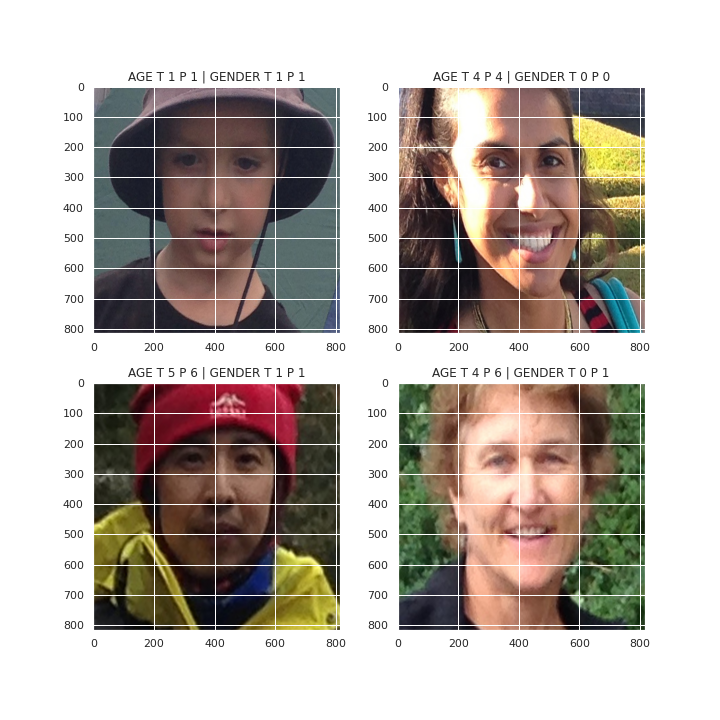
\includegraphics[width=0.9\linewidth]{images/image.png}
    \caption{Пример работы модели на 4 случайных лицах из датасета Adience}
    \label{ris:images/image.png}
\end{figure}
Здесь мы видим примеры ответов модели на случайных изображениях из датасета Adience.
Для каждого изображения написана информация про правильный ответ и ответ модели по следующему формату -
сначала идёт название целевой переменной, потом правильный ответ после метки \textbf{T}, потом ответ модели после метки \textbf{P}.
Напомним, что метки пола имеют соответствие 0 - "женщина"\,, 1 - "мужчина"\,.
Метки возраста - 0: [0, 2], 1: [4, 6], 2: [8, 12], 3: [15, 20], 4: [25, 32], 5: [38, 43], 6: [48, 53], 7: [60, 100].
    \newpage


    \section{Выводы}\label{sec:выводы}
    Решая поставленную задачу о классификации людей на фотографиях по полу и возрасту мы получили алгоритм,
    позволяющий быстро - у нас была цель суметь обрабатывать миллион фотографий за день на одной видеокарте NVIDIA RTX 2080 Ti,
    и мы ее выполнили - и качественно находить лица людей на фотографиях, а затем классифицировать их пол и возраст.
    При решении мы опробовали множество различных подходов и остановились на архитектуре RetinaFace для детектирования лиц и двух ResNet для классификации пола и возраста соответственно.
    К сожалению, мы были ограничены вычислительными и временными ресурсами, поэтому не сумели добиться действительно высокого качества.
    \newpage


    \section{Планы дальнейшей работы}\label{sec:планы-дальнейшей-работы}
    Для улучшения качества классификации в дальнейшем у нас есть несколько идей, которые мы не успели реализовать.
    В своем решении для классификации пола и возраста мы используем только лицо.
    Безусловно, лицо содержит большую часть необходимых для классификации признаков, однако используя для классификации остальные части тела, можно добиться лучших результатов.
    Также мы не умеем детектировать и классифицировать людей со спины.
    Это довольно сложная задача, но ее решение внесло бы ощутимый вклад в работу нашего алгоритма.
    Кроме этого, в конечном варианте решения мы не отсекаем лица неживых людей, найденные детектирующей моделью.
    Мы пробовали отличать живые лица от фотографий и лиц на рекламных щитах с помощью LBP~\cite{lbp},
    но такой подход не дал ожидаемых результатов и мы отложили эту задачу из-за нехватки ресурсов на ее выполнение.
    Для классификации найденных лиц на памятники и живых людей мы пробовали два подхода:
    в первом мы пытались искать отличия на основе цветовой палитры, а во втором использовали сверточные нейронные сети.
    Первый метод не показал себя достаточно хорошо, второй не удалось довести до конца из-за нехватки данных для обучения и временных ресурсов.
    \newpage


    \section{Список литературы}\label{sec:список-литературы}
    \begin{thebibliography}{0}
    \bibitem{age1994}\hypertarget{age1994}{}
    \href{https://pdfs.semanticscholar.org/20cb/d360c8e6f70aac3e11853d81e3b18e4866c2.pdf}
    {Age Classification from Facial Images.
    Young H. Kwon, Niels da Vitoria Lobo.
    In IEEE 1994}

    \bibitem{unfiltered}\hypertarget{unfiltered}{}
    \href{https://www.openu.ac.il/home/hassner/Adience/EidingerEnbarHassner_tifs.pdf}
    {Age and Gender Estimation of Unfiltered Faces.
    Eran Eidinger, Roee Enbar, Tal Hassner.
    In IEEE 2014}

    \bibitem{hassner}\hypertarget{hassner}{}
    \href{https://talhassner.github.io/home/projects/cnn_agegender/CVPR2015_CNN_AgeGenderEstimation.pdf}
    {Age and Gender Classification using Convolutional Neural Networks.
    Gil Levi, Tal Hassner.
    In IEEE 2015}

    \bibitem{INDIA}\hypertarget{INDIA}{}
    \href{https://ieeexplore.ieee.org/document/8282221}
    {Age/gender classification with whole-component convolutional neural networks (WC-CNN).
    Chun-Ting Huang, Yueru Chen, Ruiyuan Lin, C.-C. Jay Kuo.
    In IEEE 2018}

    \bibitem{smoll}\hypertarget{smoll}{}
    \href{https://merl.com/publications/docs/TR2002-12.pdf}
    {Learning Gender with Support Faces.
    Baback Moghaddam, Ming-Hsuan Yang.
    In IEEE 2002}

    \bibitem{lbp_age}\hypertarget{lbp_age}{}
    \href{https://link.springer.com/chapter/10.1007/978-3-540-74549-5_49}
    {Demographic Classification with Local Binary Patterns.
    Zhiguang Yang, Haizhou Ai. In ICB 2007}

    \bibitem{face_detection}\hypertarget{face_detection}{}
    \href{http://www.face-rec.org/algorithms/Boosting-Ensemble/16981346.pdf}
    {Robust Real-Time Face Detection.
    Paul Viola, Michael J. Jones.
    In IEEE 2003}

    \bibitem{face_detection2}\hypertarget{face_detection2}{}
    \href{http://rodrigob.github.io/documents/2014_eccv_face_detection_with_supplementary_material.pdf}
    {Face detection without bells and whistles.
    Makrus Mathias, Rodrigo Beneson, Marco Pedersoli, Lus Van Gool.
    In ECCV 2014}

    \bibitem{face_detection3}\hypertarget{face_detection3}{}
    \href{https://arxiv.org/abs/1905.01585}
    {Accurate Face Detection for High Performance.
    Faen Zhang, Xinyu Fan, Guo Ai, Jianfei Song, Yongqiang Qin, Jiahong Wu. In ArXiv 2019}

    \bibitem{resnet}\hypertarget{resnet}{}
    \href{https://arxiv.org/abs/1512.03385}
    {Deep Residual Learning for Image Recognition.
    Kaiming He, Xiangyu Zhang, Shaoqing Ren, Jian Sun.
    In IEEE 2015}

    \bibitem{align}\hypertarget{align}{}
    \href{http://www.csc.kth.se/~vahidk/papers/KazemiCVPR14.pdf}
    {One Millisecond Face Alignment with an Ensemble of Regression Trees.
    Vahid Kazemi and Josephine Sullivan.
    In IEEE 2014}

    \bibitem{lbp}\hypertarget{lpb}{}
    \href{https://arxiv.org/abs/1511.06316}
    {Face Anti-Spoofing Based on Color Texture Analysis.
    Zinelabidine Boulkenafet, Jukka Komulainen, Abdenour Hadid.
    In IEEE 2015}

    \bibitem{lbp2}\hypertarget{lpb2}{}
    \href{https://arxiv.org/abs/1803.11097}
    {Learning Deep Models for Face Anti-Spoofing: Binary or Auxiliary Supervision.
    Yaojie Liu, Amin Jourabloo, Xiaoming Liu.
    In IEEE/CVF 2018}

    \bibitem{lbp3}\hypertarget{lpb3}{}
    \href{https://arxiv.org/abs/1904.02860}
    {Deep Tree Learning for Zero-shot Face Anti-Spoofing.
    Yaojie Liu, Joel Stehouwer, Amin Jourabloo, Xiaoming Liu.
    In IEEE/CVF 2019}

    \bibitem{pfid}\hypertarget{pfid}{}
    \href{https://arxiv.org/abs/1907.02642}
    {Primate Face Identification in the Wild.
    Ankita Shukla, Gullal Singh Cheema, Saket Anand, Qamar Qureshi, Yadvendradev Jhala.
    In PRICAI 2019}

    \bibitem{pfid2}\hypertarget{pfid2}{}
    \href{https://arxiv.org/abs/1406.4773}
    {Deep Learning Face Representation by Joint Identification-Verification.
    Yi Sun, Xiaogang Wang, Xiaoou Tang.
    In NIPS 2014}

    \bibitem{pfid3}\hypertarget{pfid3}{}
    \href{https://ydwen.github.io/papers/WenECCV16.pdf}
    {A Discriminative Feature Learning Approach for Deep Face Recognition.
    Yandong Wen, Kaipeng Zhang, Zhifeng Li, and Yu Qiao.
    In ECCV 2016}

    \bibitem{densenet}\hypertarget{densenet}{}
    \href{https://arxiv.org/abs/1608.06993}
    {Densely Connected Convolutional Networks.
    Gao Huang, Zhuang Liu, Laurens van der Maaten, Kilian Q. Weinberger.
    In IEEE 2016}

    \bibitem{NUAA}\hypertarget{NUAA}{}
    \href{http://parnec.nuaa.edu.cn/xtan/data/nuaaimposterdb.html}
    {NUAA Photograph Imposter Database}

    \bibitem{lfw}\hypertarget{lfw}{}
    \href{http://vis-www.cs.umass.edu/lfw/}
    {Labeled Faces in the Wild Database}

    \bibitem{IMDB-WIKI}\hypertarget{IMDB-WIKI}{}
    \href{https://data.vision.ee.ethz.ch/cvl/rrothe/imdb-wiki/}
    {IMDB-WIKI Database}

    \bibitem{bug}\hypertarget{bug}{}
    \href{https://ibug.doc.ic.ac.uk/resources/300-W/}
    {300 Faces In-the-Wild Database}

\end{thebibliography}

\end{document}